%%%%%%%%%%%%%%%%%%%%%%%%%%%%%%%%%%%%%%%%%%%%%%%%%%%%%%%%%%%
%%%                                                     %%%
%%%   LaTeX template voor P&O: Computerwetenschappen.   %%%
%%%                                                     %%%
%%%   Schrijfopdracht 1                                 %%%
%%%                                                     %%%
%%%   7 oktober 2013                                    %%%
%%%   Versie 1.1                                        %%%
%%%                                                     %%%
%%%%%%%%%%%%%%%%%%%%%%%%%%%%%%%%%%%%%%%%%%%%%%%%%%%%%%%%%%%

\documentclass{peno-opdracht1}

\team{Indigo} % teamkleur

\begin{document}

\maketitle

Het doel van deze opdracht is een autonome zeppelin te ontwikkelen. Via de QR-codes kunnen bepaalde opdrachten aangeroepen worden.

\textbf{Fysisch ontwerp:} Houten frame met 2 grote ronde heliumballonnen, een afstandssensor (naar onder gericht), een camera (naar voren gericht) en de Raspberry Pi. De zeppelin bevat ook 2 propellers voor zijwaartse en 1 propeller voor opwaartse bewegingen.

\textbf{Software ontwerp:} Onderverdeeld in 3 delen: de GUI, de communicatie tussen GUI en Raspberry Pi en de interne programmatie op de Pi (verwerking van data van de sensoren, aansturen van de motoren).
De GUI zal in Java gemaakt worden. De communicatie tussen GUI en de Raspberry Pi zal gebeuren via een Java server-client model. Hierbij geeft de gebruiker via de GUI objecten door van klasses die opdrachten voor de Pi voorstellen (bijvoorbeeld de linkse motor gedurende 2 seconden actief). (Zie figuur \ref{schema})

Een alternatief idee was om via een webinterface te communiceren. Dit idee hebben we voorlopig aan de kant geschoven, omdat we hierover nog niet voldoende informatie hebben. Indien we hier meer over vinden, kunnen we nog omschakelen naar deze strategie.\\

\textbf{Planning:}
\begin{itemize}
\item Tegen volgende week: Uitlezen van de afstandssensor en basisontwerp van de GUI. Aangezien we nog geen volledig beeld hebben van alle onderdelen en opties, zal er telkens een nieuwe en aangepaste planning worden gemaakt.
\item De week van 21 oktober zullen we starten met eenvoudige testen, dan hebben we nog ruime tijd om eventuele problemen op te lossen.
\item De camera zal tegen de tussentijdse demo nog niet gebruikt en gemonteerd zijn, zo kunnen we ons volledig concentreren op de afstandssensor.
\end{itemize}


\textbf{Taakverdeling voor de software-onderdelen:}
\begin{itemize}
\item GUI: Dimitri Jonckers \& Wander Bavin
\item Communicatie: Sunil Tandan
\item Verwerking gegevens: Vince Goossens \& Wout Vekemans
\item Fysiek ontwerp: Wordt nog bepaald
\end{itemize}

\begin{figure}[ht!]
\centering
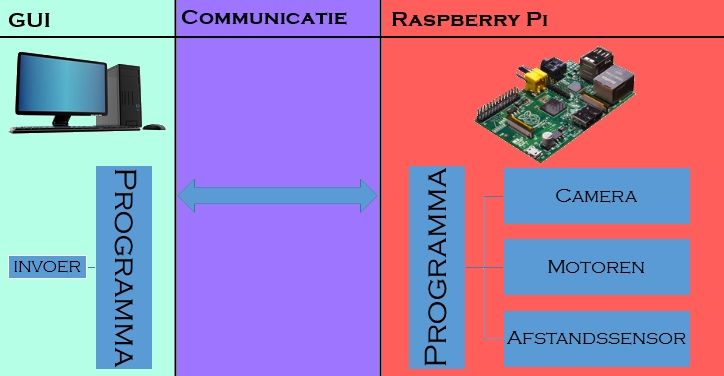
\includegraphics[height=43mm]{Schema.jpg}
\caption{Architectuur}
\label{schema}
\end{figure}






\end{document}
